\graphicspath{{chapters/04/media/}}
\chapter{Analisi dei dati}
\label{cha:analisi}
%  \begin{figure}[H]
%    \centering
%    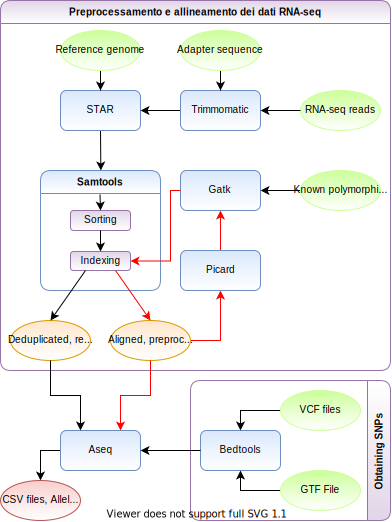
\includegraphics[scale=0.2]{pipeline.png}
%    \caption{Pipeline per l'ottenimento dei dati di allelic imbalance}
%    \label{fig:}
%  \end{figure}
\section{Conta degli SNP trovati con aseq}
\label{sec:snp_count}
Dall'esecuzione di aseq (\ref{sec:aseq}) si ottengono i valori di sbilanciamento allelico per tutti gli SNP ottenuti.
Seguendo le ``best practices'' di Gatk \cite{gatk} l'analisi \`e stata eseguita sui risultati di aseq ottenuti a partire dall'insieme dei file di allineamento generati dal processo di deduplicazione e ricalibrazione (\ref{subsec:deduprecal}).\\
Volendo considerare unicamente gli SNP presenti in eterozigosi i risultati sono filtrati considerando SNP con frazione allelica compresa tra $0.2$ e $0.8$.
Inoltre per aumentare il grado di confidenza dei risultati sono stati considerati unicamente gli SNP con un coverage\footnote{Definizione di coverage} maggiore di $10$.
Queste due operazioni di filtraggio hanno portato all'identificazione di $20895$ SNP unici, $587$ dei quali condivisi tra tutte le condizioni e replicati.\\
Come aspettato la frazione allelica degli SNP cos\`i trovati \`e distribuita secondo una normale con la media centrata a $0.5$.\\
Questa  SNP sono stati confrontati con una lista di SNP gi\`a conosciuti come eterozigoti ottenuta da cellminer \cite{cellminer}.
 \begin{figure}[H]
   \centering
   \includegraphics[scale=1]{aseq_count_2_8_10_pre.png}
	 \caption{Conta per campione degli SNP eterozigoti trovati con aseq ($0.2< af < 0.8$ e coverage $\ge 10$)}
   \label{fig:}
 \end{figure}

 %\subsection{Distribuzione degli SNP}
 %\begin{figure}[H]
   %\centering
   %\begin{tabular}{ccc}
      %\subfloat[scr DMSO]{\includegraphics[width = 0.3\textwidth]{distribution/scr_DMSO.png}} &
      %\subfloat[scr NUTLIN]{\includegraphics[width = 0.3\textwidth]{distribution/scr_NUTLIN.png}} &
      %\subfloat[shDHX30 DMSO]{\includegraphics[width = 0.3\textwidth]{distribution/shDHX30_DMSO.png}} \\
      %\subfloat[shDHX30 NUTLIN]{\includegraphics[width = 0.3\textwidth]{distribution/shDHX30_NUTLIN.png}} &
      %\subfloat[shPCBP2 DMSO]{\includegraphics[width = 0.3\textwidth]{distribution/shPCBP2_DMSO.png}} &
      %\subfloat[shPCBP2 NUTLIN]{\includegraphics[width = 0.3\textwidth]{distribution/shPCBP2_NUTLIN.png}} \\
  %\end{tabular}
   %\label{fig:}
 %\end{figure}
%
%\section{Qualit\`a dei campioni}
%Confronto tra replicato di un campione in modo da verificare come cambiano i valori di AF tra un replicato e l'altro.
 %\begin{figure}[H]
   %\centering
   %\begin{tabular}{ccc}
      %\subfloat[1 - 2]{\includegraphics[width = 0.3\textwidth]{rep_corr/scr_DMSO_TOT-rep-1-2.post.0.2.0.8.10.png}} &
      %\subfloat[1 - 3]{\includegraphics[width = 0.3\textwidth]{rep_corr/scr_DMSO_TOT-rep-1-3.post.0.2.0.8.10.png}} &
      %\subfloat[1 - 4]{\includegraphics[width = 0.3\textwidth]{rep_corr/scr_DMSO_TOT-rep-1-4.post.0.2.0.8.10.png}} \\
      %\subfloat[2 - 3]{\includegraphics[width = 0.3\textwidth]{rep_corr/scr_DMSO_TOT-rep-2-3.post.0.2.0.8.10.png}} &
      %\subfloat[2 - 4]{\includegraphics[width = 0.3\textwidth]{rep_corr/scr_DMSO_TOT-rep-2-4.post.0.2.0.8.10.png}} &
      %\subfloat[3 - 4]{\includegraphics[width = 0.3\textwidth]{rep_corr/scr_DMSO_TOT-rep-3-4.post.0.2.0.8.10.png}} \\
  %\end{tabular}
   %\label{fig:}
 %\end{figure}
%
%\section{Considerazioni sulla recalibrazione}
%\label{sec:rec_cons}
%Discussione dei risultati di ASEQ prima e dopo la recalibrazione.
 %\begin{figure}[H]
   %\centering
   %\begin{tabular}{ccc}
      %\subfloat[scr DMSO polisomale]{\includegraphics[width = 0.3\textwidth]{correlation_recal/scr_DMSO_POL_1.png}} &
      %\subfloat[scr DMSO totale]{\includegraphics[width = 0.3\textwidth]{correlation_recal/scr_DMSO_TOT_1.png}} &
      %\subfloat[scr NUTLIN polisomale]{\includegraphics[width = 0.3\textwidth]{correlation_recal/scr_NUTLIN_POL_1.png}} \\
      %\subfloat[scr NUTLIN totale]{\includegraphics[width = 0.3\textwidth]{correlation_recal/scr_NUTLIN_TOT_1.png}} &
      %\subfloat[shDHX30 DMSO polisomale]{\includegraphics[width = 0.3\textwidth]{correlation_recal/shDHX30_DMSO_POL_1.png}} &
      %\subfloat[shDHX30 DMSO totale]{\includegraphics[width = 0.3\textwidth]{correlation_recal/shDHX30_DMSO_TOT_1.png}} \\
      %\subfloat[shDHX30 NUTLIN polisomale]{\includegraphics[width = 0.3\textwidth]{correlation_recal/shDHX30_NUTLIN_POL_1.png}} &
      %\subfloat[shDHX30 NUTLIN totale]{\includegraphics[width = 0.3\textwidth]{correlation_recal/shDHX30_NUTLIN_TOT_1.png}} &
      %\subfloat[shPCBP2 DMSO polisomale]{\includegraphics[width = 0.3\textwidth]{correlation_recal/shPCBP2_DMSO_POL_1.png}} \\
      %\subfloat[shPCBP2 DMSO totale]{\includegraphics[width = 0.3\textwidth]{correlation_recal/shPCBP2_DMSO_TOT_1.png}} &
      %\subfloat[shPCBP2 NUTLIN polisomale]{\includegraphics[width = 0.3\textwidth]{correlation_recal/shPCBP2_NUTLIN_POL_1.png}} &
      %\subfloat[shPCBP2 NUTLIN totale]{\includegraphics[width = 0.3\textwidth]{correlation_recal/shPCBP2_NUTLIN_TOT_1.png}} \\
  %\end{tabular}
   %\label{fig:}
 %\end{figure}
%
\section{Ottenere i dati per gli SNP di interesse}
\label{sec:snp_filter}
La lista di SNP ottenuta dall'operazione di filtraggio dei risultati di aseq \ref{sec:snpcount} \`e stata ulteriormente confrontata con dati ottenuti da cellminer \cite{cellminer}.
Quest'ultima contiene $13681$ SNP gi\`a determinati come eterogizoti.
A partire dalla lista sono stati raccolti i dati di tutti gli SNP che rispettano le condizioni di coverage e frazione allelica in almeno $3$ replicati.
Questo viene fatto per dare forza statistica ai risultati e ridurre il rumore dovuto a errori nati dalla pipeline di analisi.\\
Per ognuno di questi SNP \`e stato svolto un t-test tra i valori di frazione allelica polisomiale e totale non corretto per test multipli.
Sono stati infine considerati significativi gli SNP con risultato del t-test inferiore a $0.05$.\\
Come si nota dalla tabella \ref{tab:significativesnp1} gli SNP significativi trovati sono $161$, dei quali $60$ nella $3'$-UTR e $8$ nella $5'$-UTR.
\begin{table}[H]
	\begin{tabular}{|c|c|c|c|}
		\hline
		Condizione & Totali & $3'$-UTR & $5'$-UTR\\
		\hline
		scr\_DMSO & $27$ & $8$ & $2$\\
		\hline
		scr\_NUTLIN & $33$ & $11$ & $2$\\
		\hline
		shDHX30\_DMSO & $22$ & $9$ & $1$\\
		\hline
		shDHX30\_NUTLIN & $25$ & $11$ & $0$\\
		\hline
		shPCBP2\_DMSO & $24$ & $10$ & $1$\\
		\hline
		shPCBP2\_NUTLIN & $30$ & $11$ & $2$\\
		\hline
	\end{tabular}
	\centering
	\label{tab:significativesnp1}
	\caption{SNP significativi per condizione}
\end{table}

\section{Caratterizzazione degli SNP di interesse}
L'ultimo passo dell'analisi \`e stata l'annotazione degli SNP in modo da determinare quali geni subiscono un cambio nel potenziale di traduzione causato da tali SNP.
L'annotazione \`e stata svolta grazie al tool snpEff \cite{snpeff}.
Confrontando i risultati dell'annotazione con una lista di geni coinvolti in molti tipi di cancro noti in letteratura si sono notati $14$ SNP che causano una variazione del potenziale di traduzione in $12$ geni.
In particolare $3$ di questi si trovano nella $3'$-UTR: \emph{rs788023} per il gene \emph{SF3B1}, \emph{rs30386} per \emph{TBC1D9B} e \emph{rs11539713} per \emph{KIF5B}.
La loro differenza nella frazione polisomiale e totale \`e descritta nei boxplot \ref{fig:SF3B1}, \ref{fig:TBC1D9B} e \ref{fig:KIF5B}.

\begin{figure}[H]
  \centering
  \includegraphics[scale=0.5]{boxplot/scr_DMSO_rs1131941.png}
  \caption{Variazione di sbilanciamento allelico tra frazione polisomiale e totale di rs788023}
  \label{fig:SF3B1}
\end{figure}

\begin{figure}[H]
  \centering
  \includegraphics[scale=0.5]{boxplot/scr_DMSO_rs1131941.png}
  \caption{Variazione di sbilanciamento allelico tra frazione polisomiale e totale di rs30386}
  \label{fig:TBC1D9B}
\end{figure}

\begin{figure}[H]
  \centering
  \includegraphics[scale=0.5]{boxplot/scr_DMSO_rs1131941.png}
  \caption{Variazione di sbilanciamento allelico tra frazione polisomiale e totale di rs11539713}
  \label{fig:KIF5B}
\end{figure}



\section{Conclusioni}
\label{sec:ending}
